% Technical system architecture, vertical (top-to-bottom) single-column layout (8.6 cm wide). Compiled standalone to fig_architecture.pdf;
% a 300 dpi PNG is made for the Word builds. Included at \columnwidth (IEEE) or a fixed width (ERIS).
\documentclass[tikz,border=2pt]{standalone}
\usetikzlibrary{positioning,arrows.meta,fit,backgrounds,calc}
\usepackage{amsmath}
\begin{document}
\sffamily
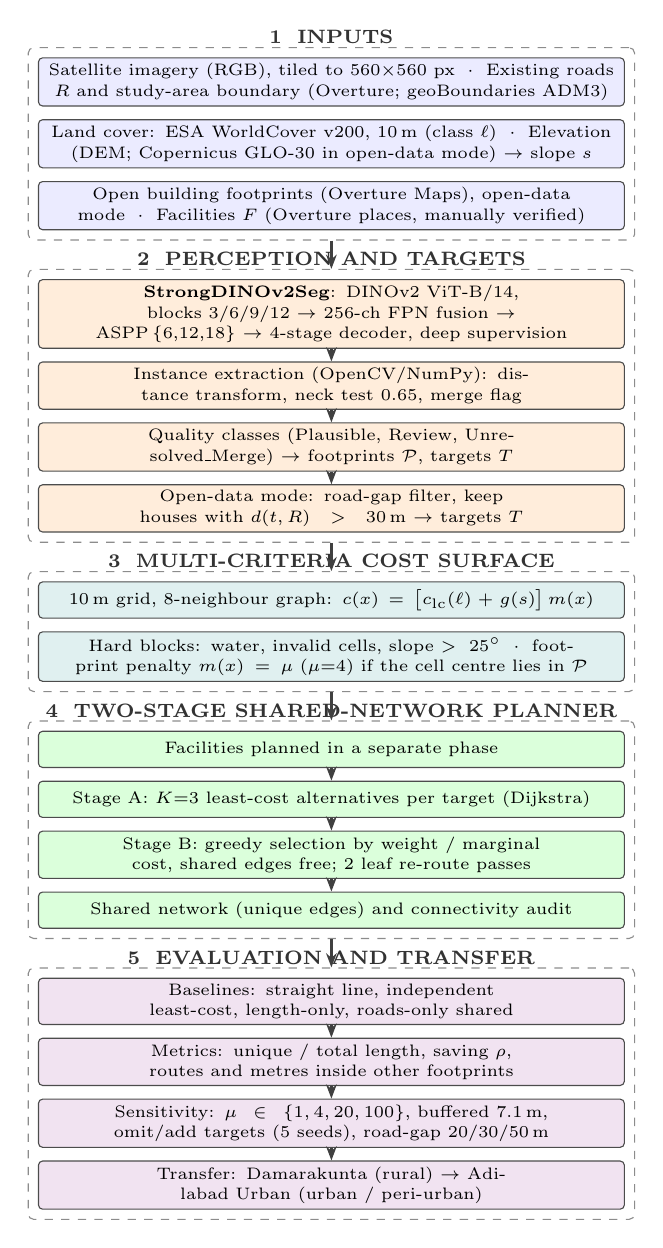
\begin{tikzpicture}[node distance=0.16cm]
\tikzset{
  blk/.style={draw=black!70,rounded corners=1.5pt,align=center,inner sep=2pt,font=\fontsize{6.4}{7.4}\selectfont,text width=7.3cm,minimum height=0.46cm},
  inp/.style={blk,fill=blue!8},
  per/.style={blk,fill=orange!14},
  cst/.style={blk,fill=teal!12},
  pln/.style={blk,fill=green!14},
  evl/.style={blk,fill=violet!11},
  arr/.style={-{Stealth[length=1.8mm]},thick,black!75},
  grp/.style={draw=black!45,dashed,rounded corners=2pt,inner sep=3.5pt},
  ttl/.style={font=\fontsize{6.6}{7.6}\selectfont\bfseries,text=black!80,fill=white,inner sep=1pt}
}
% --- stage 1: inputs
\node[inp] (i1) {Satellite imagery (RGB), tiled to $560{\times}560$ px\; $\cdot$\; Existing roads $R$ and study-area boundary (Overture; geoBoundaries ADM3)};
\node[inp,below=of i1] (i2) {Land cover: ESA WorldCover v200, 10\,m (class $\ell$)\; $\cdot$\; Elevation (DEM; Copernicus GLO-30 in open-data mode) $\rightarrow$ slope $s$};
\node[inp,below=of i2] (i3) {Open building footprints (Overture Maps), open-data mode\; $\cdot$\; Facilities $F$ (Overture places, manually verified)};
\begin{scope}[on background layer]\node[grp,fit=(i1)(i3),label={[ttl]above:1\; INPUTS}] (g1) {};\end{scope}
% --- stage 2: perception
\node[per,below=0.62cm of i3] (p1) {\textbf{StrongDINOv2Seg}: DINOv2 ViT-B/14, blocks 3/6/9/12 $\rightarrow$ 256-ch FPN fusion $\rightarrow$ ASPP\,\{6,12,18\} $\rightarrow$ 4-stage decoder, deep supervision};
\node[per,below=of p1] (p2) {Instance extraction (OpenCV/NumPy): distance transform, neck test $0.65$, merge flag};
\node[per,below=of p2] (p3) {Quality classes (Plausible, Review, Unresolved\_Merge) $\rightarrow$ footprints $\mathcal P$, targets $T$};
\node[per,below=of p3] (p4) {Open-data mode: road-gap filter, keep houses with $d(t,R)>30$\,m $\rightarrow$ targets $T$};
\begin{scope}[on background layer]\node[grp,fit=(p1)(p4),label={[ttl]above:2\; PERCEPTION AND TARGETS}] (g2) {};\end{scope}
% --- stage 3: cost surface
\node[cst,below=0.62cm of p4] (c1) {10\,m grid, 8-neighbour graph: $c(x)=\bigl[c_{\mathrm{lc}}(\ell)+g(s)\bigr]\,m(x)$};
\node[cst,below=of c1] (c2) {Hard blocks: water, invalid cells, slope $>25^{\circ}$\; $\cdot$\; footprint penalty $m(x)=\mu$ ($\mu{=}4$) if the cell centre lies in $\mathcal P$};
\begin{scope}[on background layer]\node[grp,fit=(c1)(c2),label={[ttl]above:3\; MULTI-CRITERIA COST SURFACE}] (g3) {};\end{scope}
% --- stage 4: planner
\node[pln,below=0.62cm of c2] (s0) {Facilities planned in a separate phase};
\node[pln,below=of s0] (s1) {Stage A: $K{=}3$ least-cost alternatives per target (Dijkstra)};
\node[pln,below=of s1] (s2) {Stage B: greedy selection by weight / marginal cost, shared edges free; 2 leaf re-route passes};
\node[pln,below=of s2] (s3) {Shared network (unique edges) and connectivity audit};
\begin{scope}[on background layer]\node[grp,fit=(s0)(s3),label={[ttl]above:4\; TWO-STAGE SHARED-NETWORK PLANNER}] (g4) {};\end{scope}
% --- stage 5: evaluation
\node[evl,below=0.62cm of s3] (e1) {Baselines: straight line, independent least-cost, length-only, roads-only shared};
\node[evl,below=of e1] (e2) {Metrics: unique / total length, saving $\rho$, routes and metres inside other footprints};
\node[evl,below=of e2] (e3) {Sensitivity: $\mu\in\{1,4,20,100\}$, buffered 7.1\,m, omit/add targets (5 seeds), road-gap 20/30/50\,m};
\node[evl,below=of e3] (e4) {Transfer: Damarakunta (rural) $\rightarrow$ Adilabad Urban (urban / peri-urban)};
\begin{scope}[on background layer]\node[grp,fit=(e1)(e4),label={[ttl]above:5\; EVALUATION AND TRANSFER}] (g5) {};\end{scope}
% --- flows between stages and inside stages
\draw[arr] (g1.south) -- (g2.north);
\draw[arr] (g2.south) -- (g3.north);
\draw[arr] (g3.south) -- (g4.north);
\draw[arr] (g4.south) -- (g5.north);
\foreach \a/\b in {p1/p2,p2/p3,p3/p4,s0/s1,s1/s2,s2/s3,e1/e2,e2/e3,e3/e4} \draw[arr] (\a) -- (\b);
\end{tikzpicture}
\end{document}
